\documentclass[12pt]{article}
\usepackage[T1]{fontenc}
\usepackage[spanish]{babel}
\usepackage{listings}
\usepackage{graphicx}
\usepackage{float}
\graphicspath{ {./figuras/} }

\lstset{
literate=
 {á}{{\'a}}1 
 {ã}{{\~a}}1 
 {é}{{\'e}}1 
 {ó}{{\'o}}1
 {ú}{{\'u}}1
 {ñ}{{\~n}}1
 {í}{{\'i}}1
 %extend the list as needed
 }

\title{Proyecto Final de Informática}
\author{Julian Rodríguez Vega, Dayanna Lugo Vargas y Maria Fernanda Marin}
\date{Agosto 2021}

\begin{document}

\begin{titlepage}
\maketitle
\end{titlepage}

\section{Menú}

Iniciando con el menú de inicio, con un ciclo \verb+do while+ o un ciclo \verb+while+, junto a una variable de tipo booleana, es posible programar un programa por consola que pueda continuar corriendo constantemente.

\begin{lstlisting}[language=c++]
int main(){
    bool run = true;
    do {
        // Programa
    } while(run);
    return 0;
}
\end{lstlisting}

Dentro de este ciclo  sera necesario cambiar el valor de \verb+run+, para salir del ciclo y terminar la ejecución del programa.

\begin{figure}[h]
    \caption{Diagrama de Flujo del Ciclo para un Menú}
    \centering
    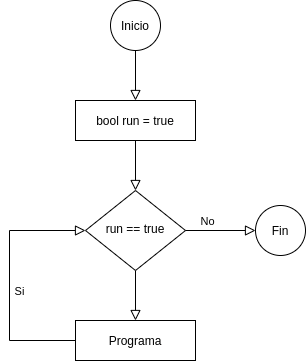
\includegraphics[scale=0.5]{menu_loop.png}
\end{figure}

Con una variable programa se captura que programa el usuario desea ejecutar, esta variable es evaluada con un switch envez de agrupar multiples condicionales.

\begin{lstlisting}[language=c++]

cout << "Programas Disponibles" << endl;
cout << "1. Calculador de Promedio" << endl;
cout << "2. Contador de Digitos." << endl;
cout << "3. Sucesión Numerica." << endl;

int programa;
cout << "Ingrese una opción: ";
cin >> programa;

switch(programa) {
    case 1:
        // Programa Calculador de promedio
        break;
    case 2:
        // Programa Contador de Digitos
        break;
    case 3:
        // Programa Susesión Numerica
        break;
    default:
        cout << "Esa no es una opción valida";
}
\end{lstlisting}

En el caso \verb+default+ cuando el usuario no ingrese una de las 3 opciones, sera entonces dirigido a un ciclo para terminar la ejecución del programa. Cuando termine de ejecutarse el \verb+switch+, el ciclo del menu inicial continuara ejecutando y el usuario podra escoger otro programa por ejecutar.

\begin{figure}[H]
    \caption{Diagrama de Flujo de Switch para Escoger Programas}
    \centering
    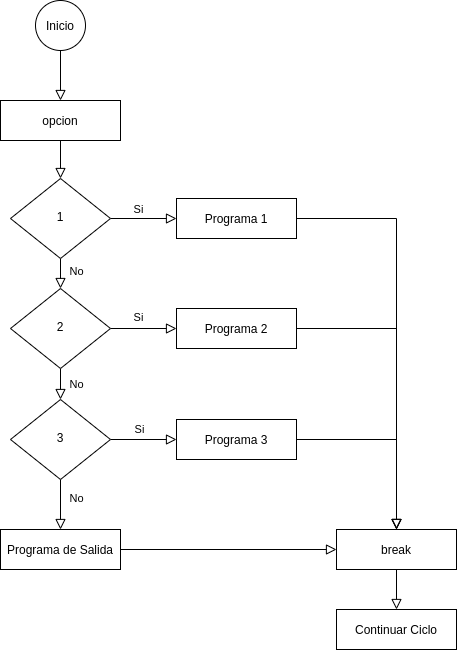
\includegraphics[scale=0.4]{switch_menu.png}
\end{figure}


\section{Programa Contador de Dígitos}

El segundo programa en el enunciado solicita mostrar la cantidad de dígitos en un numero y la suma de los mismos, este valor puede ser almacenado en una variable de tipo \verb+string+ la cual se encuentra compuesta por un conjunto de caracteres sobre los cuales se puede iterar. Para revisar la cantidad de caracteres dentro de una cadena de texto es posible utilizar la función \verb+length()+, la cual esguardada en una nueva variable y usada para validar la cantidad de dígitos en el numero con un condicional, en donde, de ser un numero valido se continuara con el ciclo sino se mostrara un mensaje de error y el usuario sera dirigido al menu principal.

\begin{figure}[H]
    \caption{Diagrama de Flujo de la Validación en el Contador de Dígitos}
    \centering
    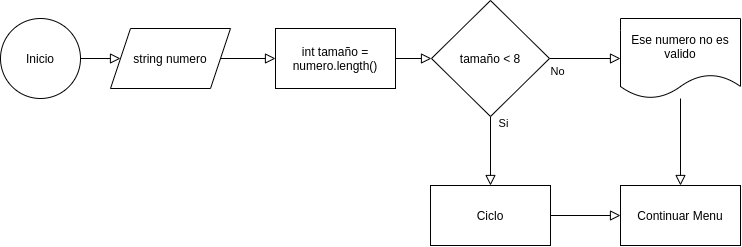
\includegraphics[scale=0.5]{programa2_validacion.png}
\end{figure}

Para este ciclo se utilizara un ciclo \verb+for+ y una variable temporal para guardar el valor del carácter por el cual se esta iterando en el ciclo, puesto que esta variable sera de tipo \verb+string+, sera necesario convertirla a \verb+integer+ con la función \verb+stoi+ y así incrementar la variable con la suma de los dígitos.


\begin{lstlisting}[language=c++]
cout << "Contador de Dígitos" << endl;
string numero;
// Capturar la entrada
cout << "Ingrese un numero:" << "";
cin >> numero;
int tamaño = numero.length();
// Con la funcion length es posible obtner el tamaño de una cadena de texto
if(tamaño < 8) {
    // Variables acumuladores
    int suma = 0;
    // Variable temporal para guardar el valor de un item dentro de la cadena de texto
    string temp;
    // Iterar por cada item en la cadena de texto
    for(int i = 0; i < tamaño; i++){
        // Guardar el valor actual
        temp = numero[i];
        suma = suma + stoi(temp);
    }
    // Mostrar resultados
    cout << "- Suma de los digitos: " << suma << endl;
    cout << "- Cantidad de digitos: " << tamaño << endl;
} else {
    cout << "Ese numero no es valido" << endl;
}
\end{lstlisting}

\begin{figure}[H]
    \caption{Diagrama de Flujo del Ciclo para Sumar Dígitos en un Numero}
    \centering
    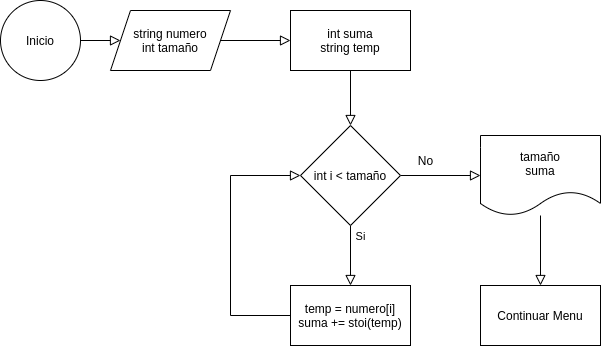
\includegraphics[scale=0.5]{programa2_ciclo.png}
\end{figure}


\end{document}
